\documentclass[10pt,twocolumn,letterpaper]{article}

\usepackage{cvpr}
\usepackage{times}
\usepackage{epsfig}
\usepackage{graphicx}
\usepackage{amsmath}
\usepackage{amssymb}
\usepackage{float}
\usepackage{url}
\usepackage{subcaption}

% Include other packages here, before hyperref.

\usepackage[breaklinks=true,bookmarks=false]{hyperref}

\cvprfinalcopy

\def\httilde{\mbox{\tt\raisebox{-.5ex}{\symbol{126}}}}

\begin{document}

\title{Geneus: Taxonomic Classification from Species Descriptions}

\author{Jason Dong, Yidi Huang, Mark Lalor, Andrew Tarnoff, Hung Vu \\
Case Western Reserve University\\
10900 Euclid Ave, Cleveland, OH 44106\\
{\tt\small \{jwd67, yidi, mwl58, art81, hdv4\}@case.edu}}

\maketitle

\begin{abstract}
   Deep learning has many applications in different fields such as computer vision, speech recognition, natural language processing, medical image analysis. Wikipedia has also been a great source of information for years and its information on each page can be a valuable and interesting data to apply to a deep learning model. In this project, we want to apply the richness of information on each species’ Wikipedia page to classify its biological taxonomy. We use two language modeling approaches to predict the taxonomy of an organism based on a short description. We find that our approaches perform well for distinguishing between kingdoms. Our code can be found at \url{https://github.com/dongjason1/Geneus}. 
\end{abstract}

\section{Introduction}

    In biology, taxonomy is used to define and classify groups of biological organisms on the basis of shared characteristics. The principle of ranking has changed over the years, but in this paper, we will be using the modern principal ranks which are domain, kingdom, phylum, class, order, family, genus, and species (Figure \ref{fig:taxonomy_ranks}). In this project, we want to build a deep learning model to classify the biological taxonomy of each species on Wikipedia page. In each species’ Wikipedia page, there is always a scientific classification for that specific species. For example, figure \ref{fig:wolf} is the scientific classification for Wolf. Wolf's kingdom is classified as Animala, phylum as Chordata, class as Mammalia, order as Carnivora, family as Canidae, genus as Canis, and spcies as C. lupus . Using the texts from Wikipedia that describe the characteristics of each species, we hope to extract a meaningful yet consolidate text representation and feed it to our deep learning model.
    
    It's interesting if we can see a correlation between descriptions of an animal and the scientific classification of the animal. Since Wikipedia is the mix of relevant and irrelevant data, it's harder to use those data to classify the species. However, if we can scrape the Wikipedia page of the species and get a handful of meaning words, we will be able to classify the species.

\begin{figure}
  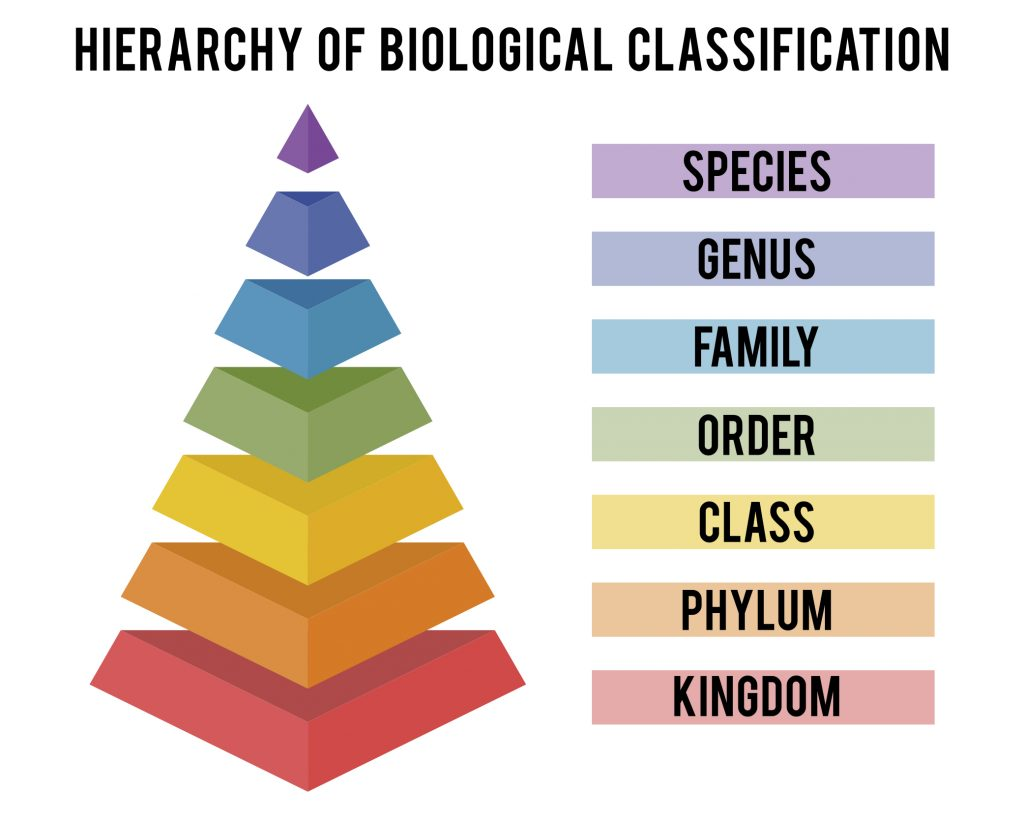
\includegraphics[width=\linewidth]{taxonomy-1024x819.jpg}
  \caption{Hierarchy of biological classification}
  \label{fig:taxonomy_ranks}
\end{figure}

\begin{figure}
  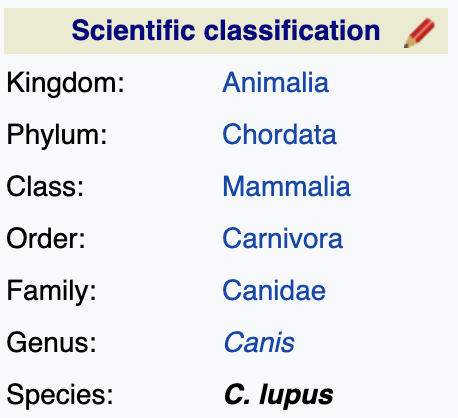
\includegraphics[width=\linewidth]{wolf.png}
  \caption{Full taxonomic classification of Wolf}
  \label{fig:wolf}
\end{figure}

\section{Background}

    In order to pull out a specific information from a mixture of relevant and irrelevant data, we will use Natural Language Processing to extract information from a general block of text. Pre-trained language model has been proven to be very effective to improve many natural language processing tasks. We will use the word extracted from YAKE (Yet Another Keyword Extractor) by Campos et al \cite{article} and the word embeddings provided by pre-trained BERT (Bidirectional Encoder Representations from Transformers) model by Google \cite{devlin2018bert}. (Figure \ref{fig:bert_des}) After getting the word representations, we will use them as input of our deep learning model to classify the taxonomy of each species. It's noteworthy that we need to make sure the text representations from those pre-trained models do not contain any labels that we will classify in the future.

    \begin{figure}
        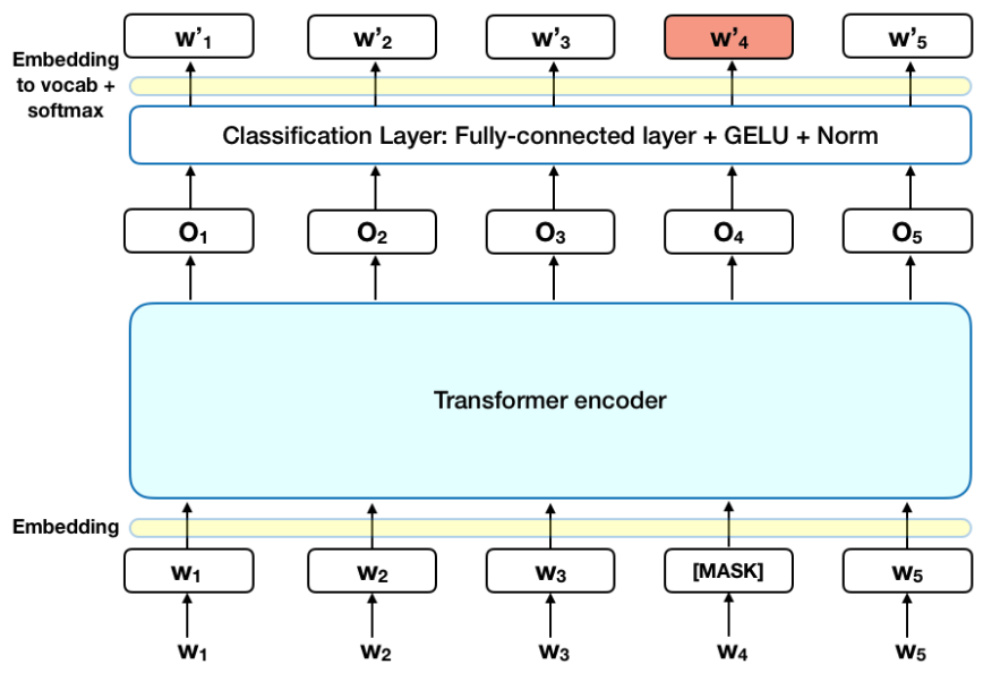
\includegraphics[width=\linewidth]{bert_des.png}
        \caption{BERT by Google}
        \label{fig:bert_des}
    \end{figure}
\section{Data}

\begin{figure}
  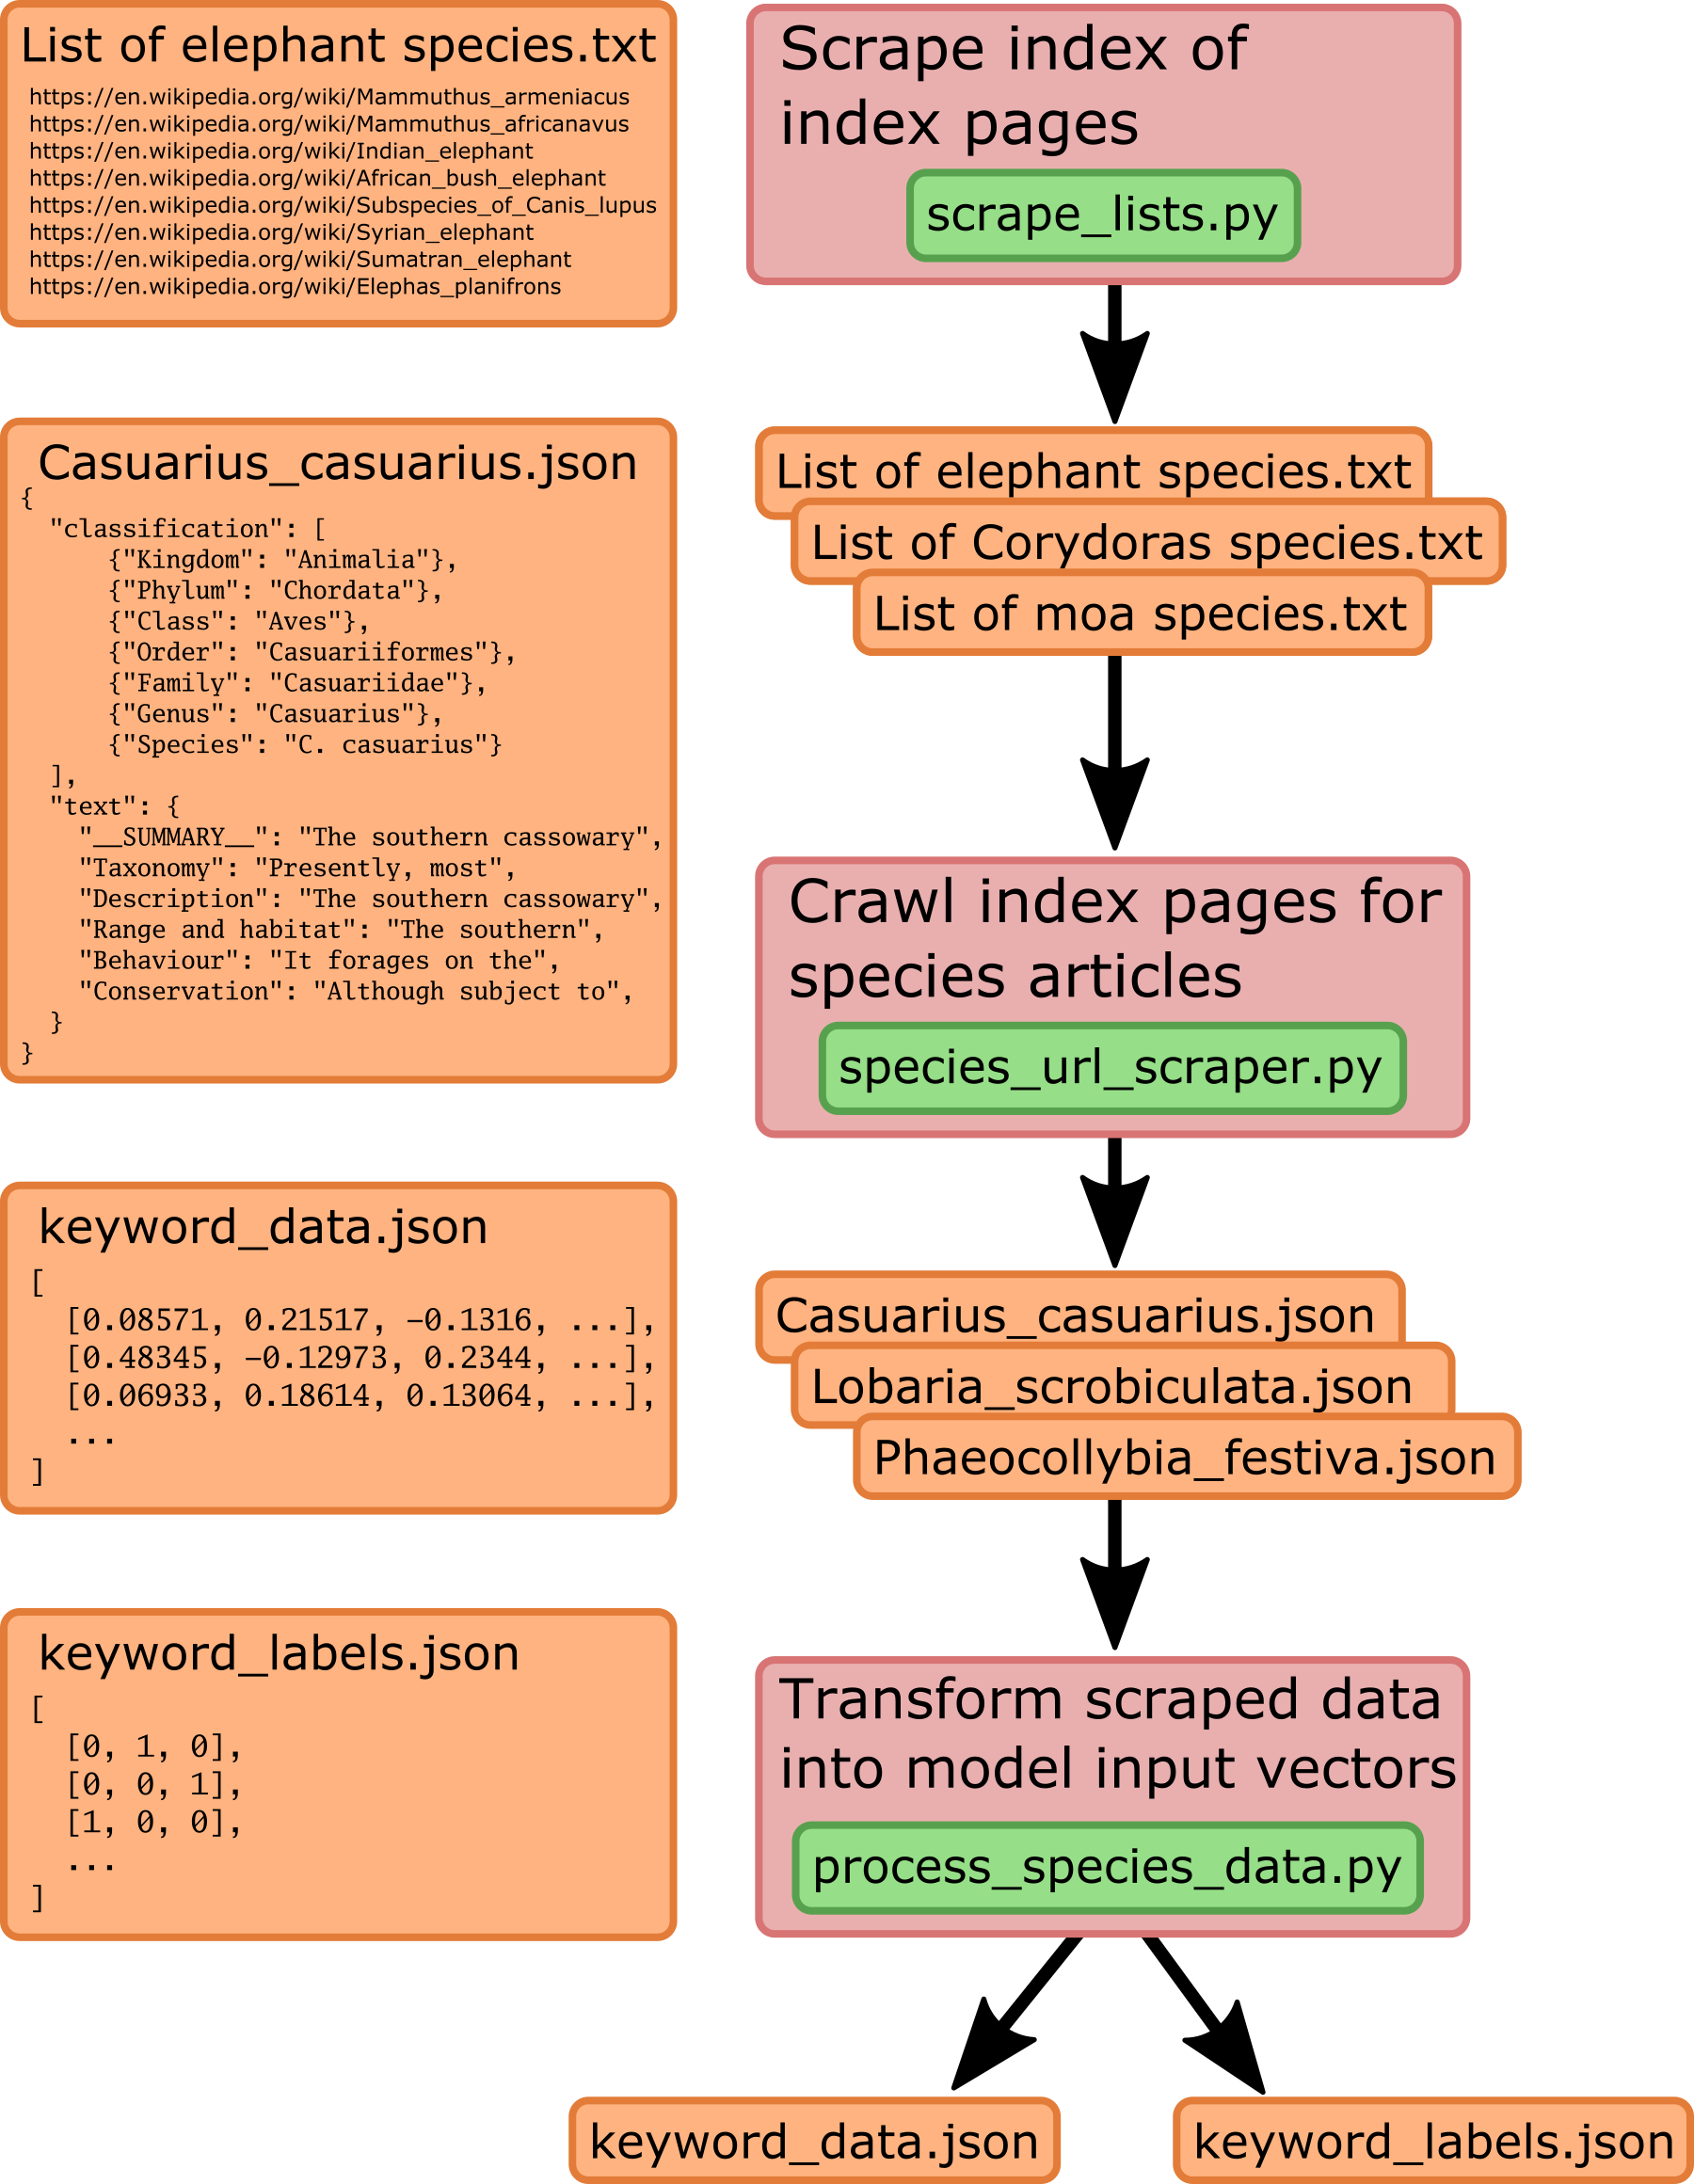
\includegraphics[width=\linewidth]{data.png}
  \caption{Visualization of the data-processing pipeline.}
  \label{fig:data}
\end{figure}

A flowchart of the data collection and processing pipeline can be seen in Figure \ref{fig:data}. The process involves collecting data from Wikipedia and then processing it into representations that will be used as inputs for the deep learning model.

We leveraged Python scripts for their simplicity and the availability of relevant libraries. 

\subsection{Scrape index pages}
The first step is to creates lists of species articles which is done by supplying manually-found species index pages using \texttt{species\_url\_scraper.py} which then scrapes these articles to output lists of Wikipedia article URLs. This scraping is done with an HTML parser that searches for hyperlinks that match the \texttt{https://en.wikipedia.org/wiki/Article} form. These are then checked to ensure they actually correspond to an organism. This step outputs a collection of URLs of these articles.

\subsection{Scrape species articles}
The next step consumes these URL lists and scrapes the Wikipedia pages to extract the scientific classification as well as the text content from each of the sections. The scraping parses the classification from the info boxes on the side of all the pages, which are very consistently-structured across all of English Wikipedia. The text content of various sections is retrieved reliably using the Wikipedia API.

\subsection{Create input vectors}
The final step of the data process involves loading all of the crawled data into memory to create our final training data and labels. We take the raw data and apply functions to create training data and training labels. We work with two different functions to create our data which is detailed in Section \ref{section:methods}.

\subsection{Review Collected Data}

We selected animal, plant, and fungi pages to scrape (we decided to not work with unicellular organisms simply because they are vastly different from multicellular ones). We ultimately collected data for 25474 species-level pages (5926 animal, 16574 plant, and 2974 fungi). 

We took a lot at our data by observing the sizes of key parts of the articles by plotting histograms as seen in Figure \ref{fig:article_lengths}. Every Wikipedia article has a "summary" which is the initial text without any particular header. There are many "stub" articles with very few words in the summary and little total content. An extremely common first section for species articles was "Description" (10070/25474 articles contained this section). Much like the summaries we note that there is a large number of small descriptions, but the large majority of descriptions are medium-to-large in length, a good sign that this data is going to be useful.

\begin{figure}
  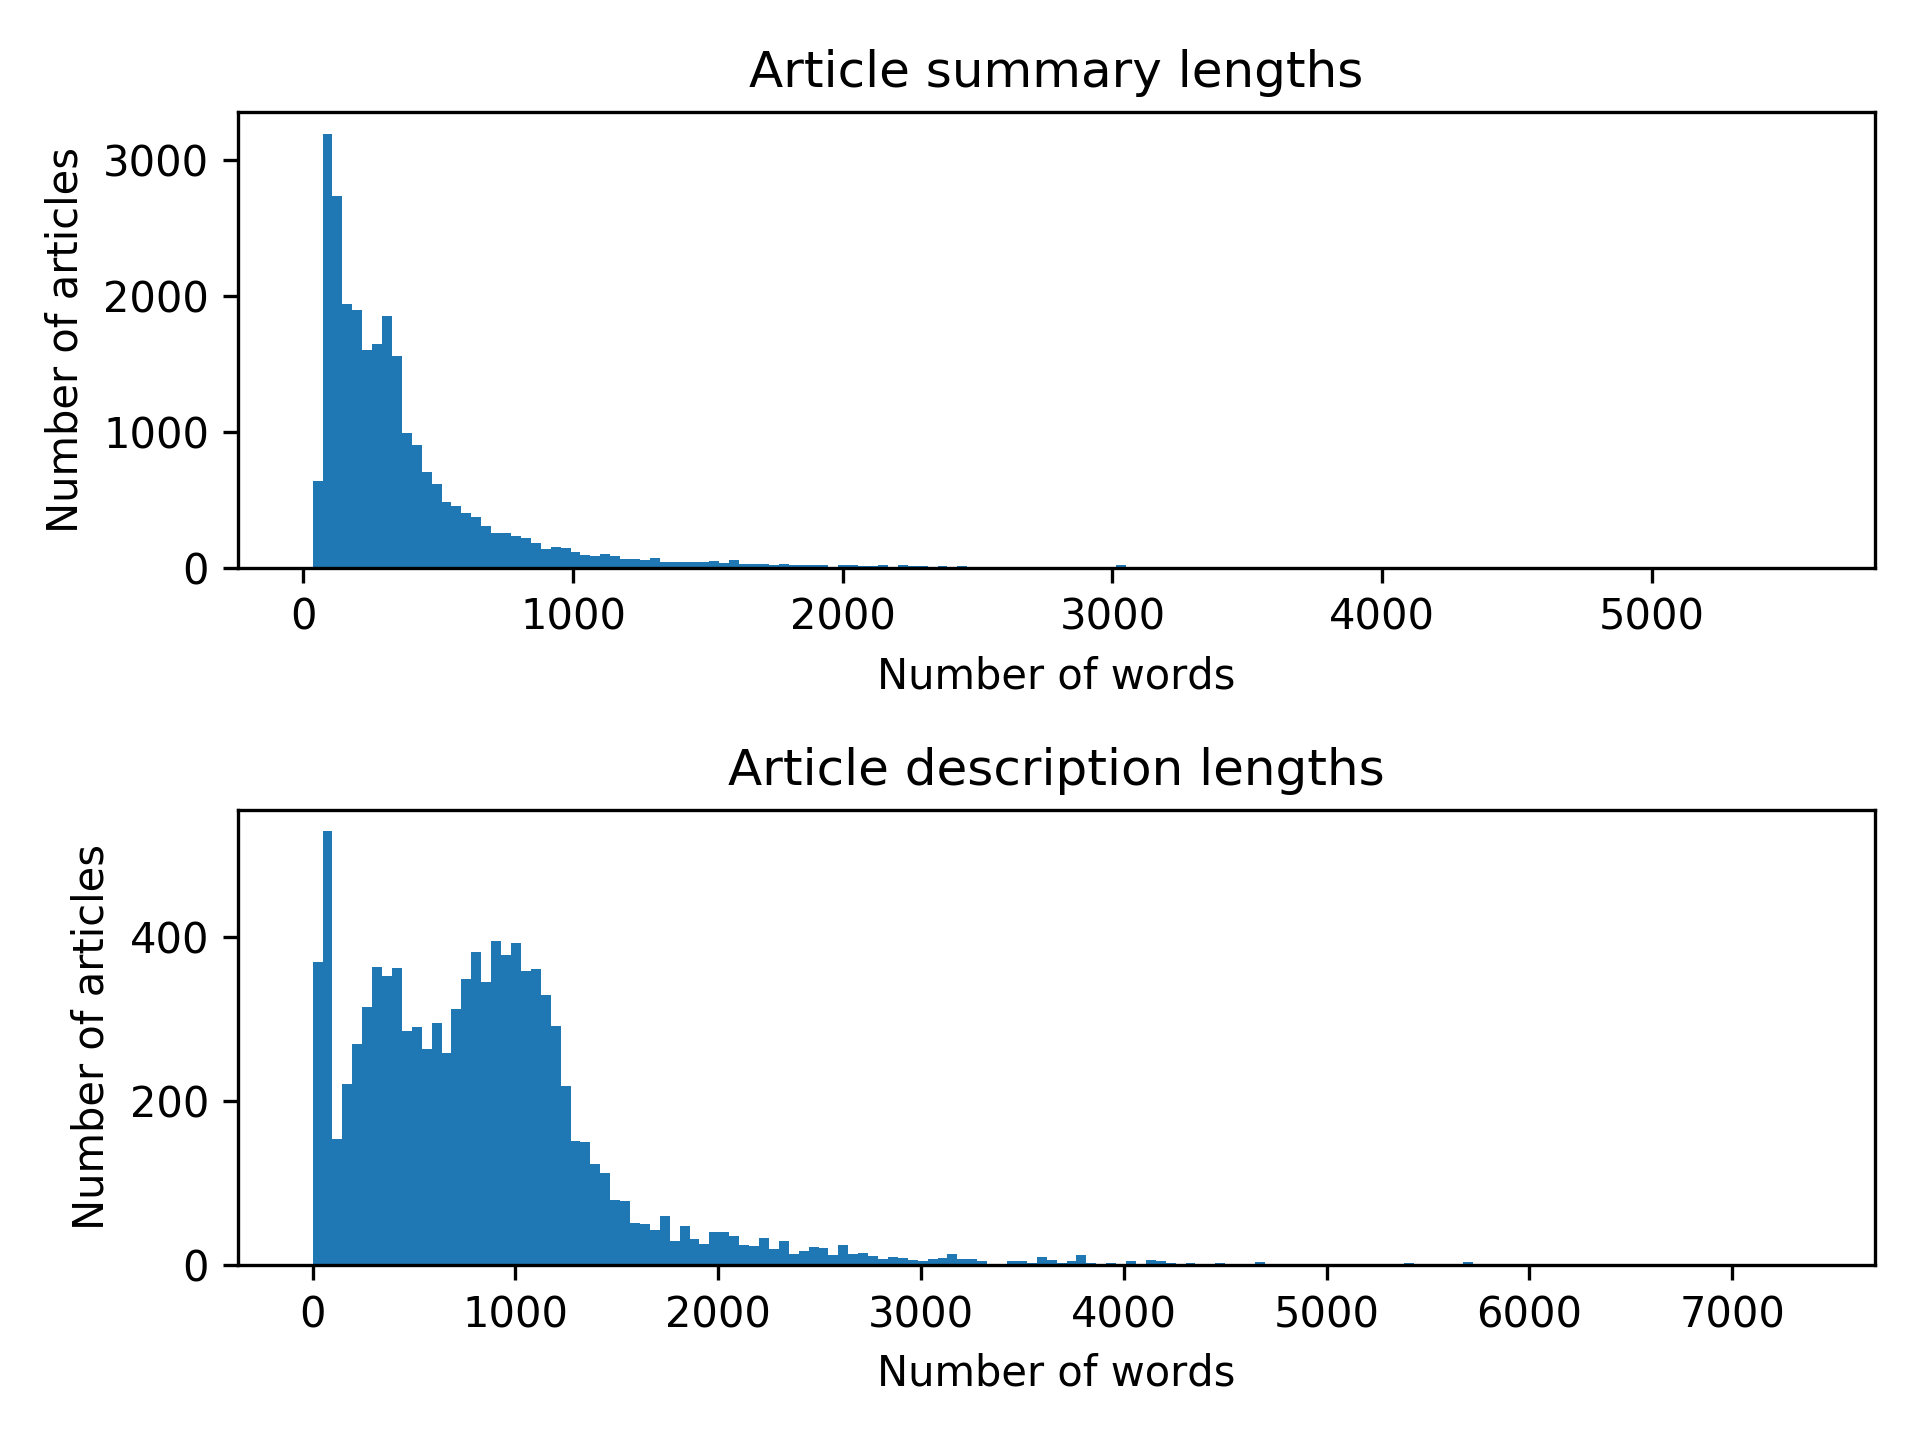
\includegraphics[width=\linewidth]{article_lengths.png}
  \caption{Histograms for article summary and description lengths.}
  \label{fig:article_lengths}
\end{figure}

With more time, we would have liked to experiment with filtering on the data to remove articles with certain characteristics, for example we could filter a decent amount of articles with extremely short summaries or descriptions without. Filtering to only use articles that contain descriptions is another experiment that we hypothesize may improve results at the expense of discarding over half of the scraped articles. 

\section{Methods}
\label{section:methods}

Our overall pipeline is summarized in Figure \ref{fig:classifier_overview}. We decided to try two different natural language processing methods to generate representations of the data. The first was a simple keyword extractor followed by a pre-trained word embedding model. The other was BERT, the Bidirectional Encoder Representations from Transformers model by Google. These vectorized representations could then be easily fed into a feed forward model for training. For testing, we withheld some of the testing data for cross validation and we attempted to write our own paragraphs to see if the model could predict the taxonomy we were thinking of. 

\begin{figure}[h]
  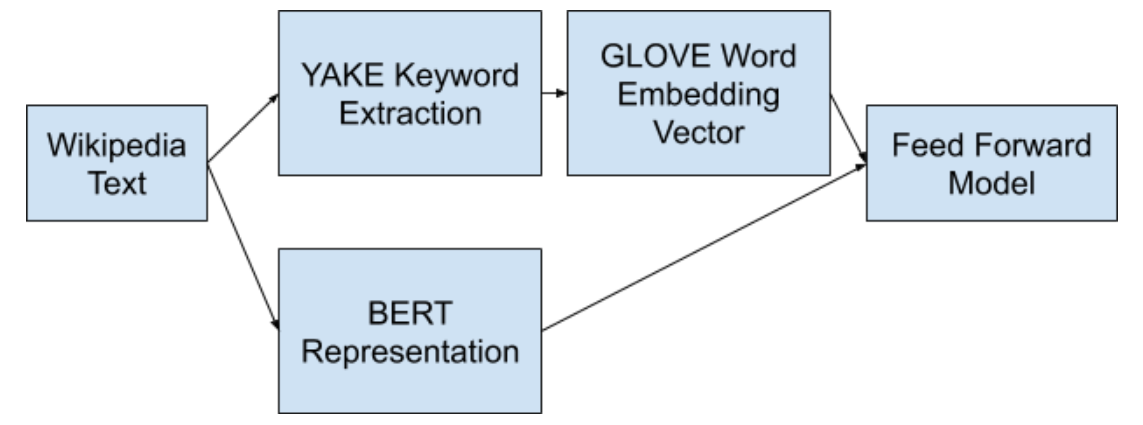
\includegraphics[width=\linewidth]{classifier_overview.png}
  \caption{Flowchart of our classifier.}
  \label{fig:classifier_overview}
\end{figure}

\subsection{Keyword Extraction}
We decided to use YAKE, Yet Another Keyword Extractor by Campos et al \cite{article}. Using PKE, the Python Keyphrase Extraction module \cite{boudin:2016:COLINGDEMO}, we tested several keyword extractors and chose YAKE for its simplicity and proven success. We fed the pretrained model our wikipedia texts and it returned the top 20 keywords and their relevancy scores. 

\begin{figure*}
  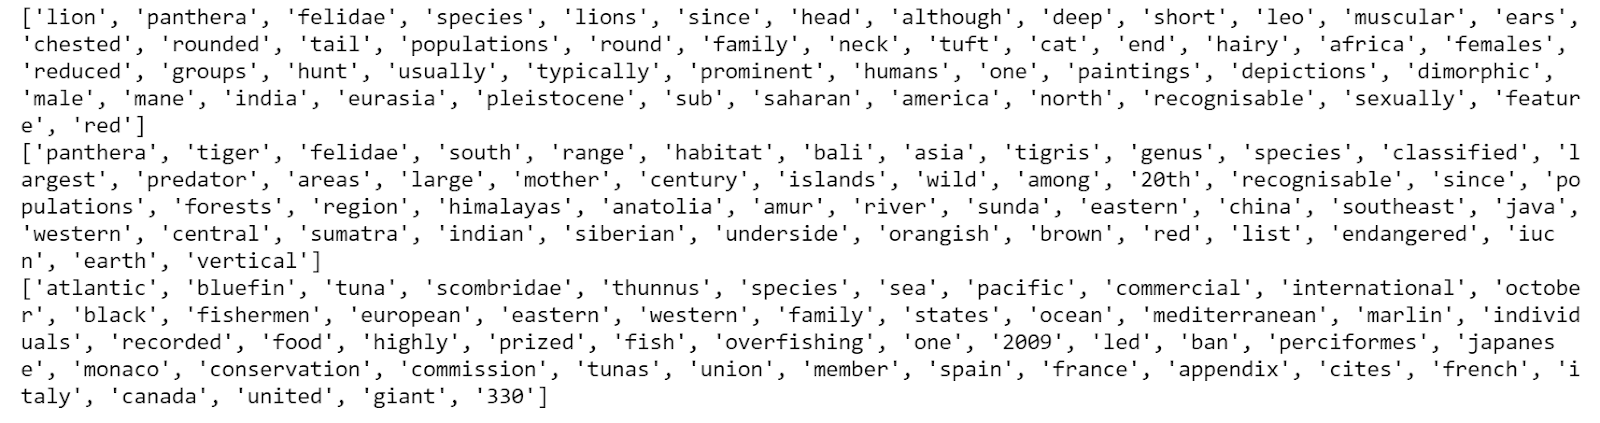
\includegraphics[width=\linewidth]{keywords_example.png}
  \caption{Examples of keywords extracted from the lion, tiger, and bluefin tuna wikipedia pages.}
  \label{fig:keywords_example}
\end{figure*}

To vectorize our keywords, we used the pre-trained word embeddings model, GloVe or Global Vectors for Word Representation \cite{pennington2014glove}. The model was pretrained on 2014 wikipedia data which made it suitable for representing our input. In testing, we discovered some words in our data had not been seen by GloVe and we were unable to vectorize it. We decided to remove those words from our training data because it rarely occurred and the pretrained model was able to generate vectors for most of our keywords. A possible alternative would be to train our own GloVe model based on the data we have. 

After vectorizing the keywords, we used a weighted sum of the vectors based on their relevancy scores. Our first attempt to directly sum the vectors resulted in vectors that were all very similar to each other. We attribute this to some common words that are irrelevant to species taxonomy pushing the vectors in a common direction since most wikipedia descriptions use similar language. Our weighted sum approach seemed to overcome this. We multiplied the keyword vectors by its relevancy scores scaled. In other words, the sum of the relevancy scores equalled 1. As a result of this however, our representation varied from the GloVe representation and applying the word embeddings map in the other direction gave irrelevant results. However, from testing different animal species, we saw a good correlation between similar species. As an example, using Euclidean distance as our distance metric, we found that the Lion vector was close to the Tiger vector, but both were far from Bluefin Tuna. This result led us to believe that we have successfully created a representation that stores the characteristics associated with different species. 

\subsection{BERT}
Bidirectional Encoder Representations from Transformers (BERT) is a language model developed by Devlin et al \cite{devlin2018bert}. It is capable of state of the art performance on a number of language tasks including the Stanford Question and Answer Dataset (SQuAD) and several tasks from General Language Understanding and Evaluation (GLUE) suite. The BERT model is first pre-trained using a pair of unsupervised tasks. In the masked LM task, a small proportion of the training tokens are hidden at random, and the model is tasked with predicting the masked tokens. In the next sentence prediction task, pairs of sentences (A,B) are fed as input, and the model is tasked with predicting whether sentence B naturally follows sentence A. The resulting pre-trained model can either be fine-tuned for specific language tasks, or can be used to produce general language embeddings for text passages. 

\begin{figure}
  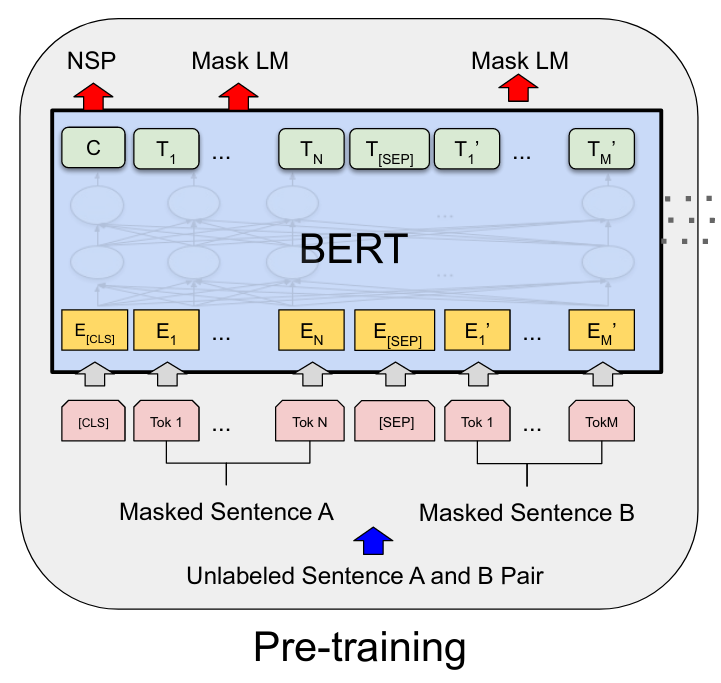
\includegraphics[width=\linewidth]{bert_pretrain.png}
  \caption{Schematic of BERT pre-training.}
  \label{fig:bert_pretrain}
\end{figure}

Given our limited sample size, we chose to use embeddings produced by the pre-trained BERT model rather than fine-tuning the entire model. We use a 24-layer model which has 340M total parameters and hidden representations of size 1024, retrieved from Tensorflow hub \cite{tfHub}. This model was configured with a 128-token maximum input size. Inputs were first tokenized using the BERT tokenizer, then the first 126 input tokens were used by prepending and appending the \texttt{[CLS]} and \texttt{[SEP]} tokens, respectively. The tokenized input was fed into BERT, and the embedding of the \texttt{[CLS]} token used as the passage representation. 

\subsection{Model}

The classification network that we used to predict the kingdom/phylum from the representations described above consisted of 2 hidden layers and was a simple dense, feed-forward network. We decided to use ReLU activation functions for the hidden layers and softmax activations for the output layer. Also, to test how it would affect our results, we decided to try slightly different configurations of these networks by changing the number of neurons in each of the hidden layers and/or by reducing the number of hidden layers to 1. We used 3 different configurations and they are outlined in figure \ref{fig:keyword_model} \ref{fig:bert_model} below

\begin{figure}
\begin{subfigure}{\linewidth}
  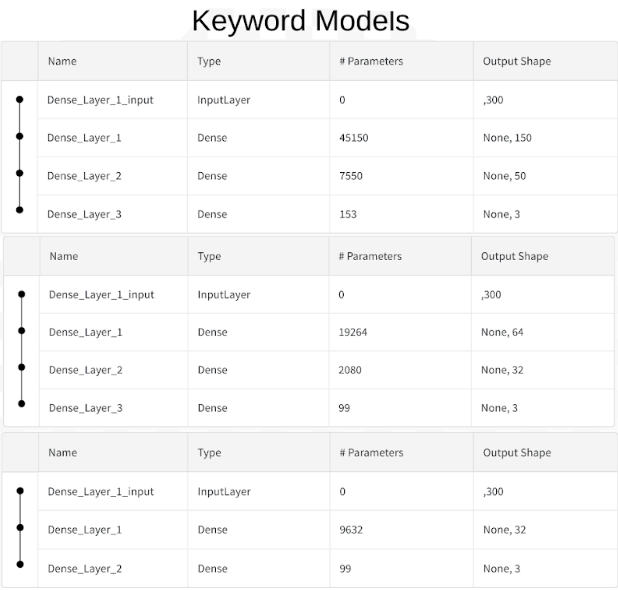
\includegraphics[width=\linewidth]{keyword_model}
  \caption{Keyword model configuration}
  \label{fig:keyword_model}
\end{subfigure}
\begin{subfigure}{\linewidth}
  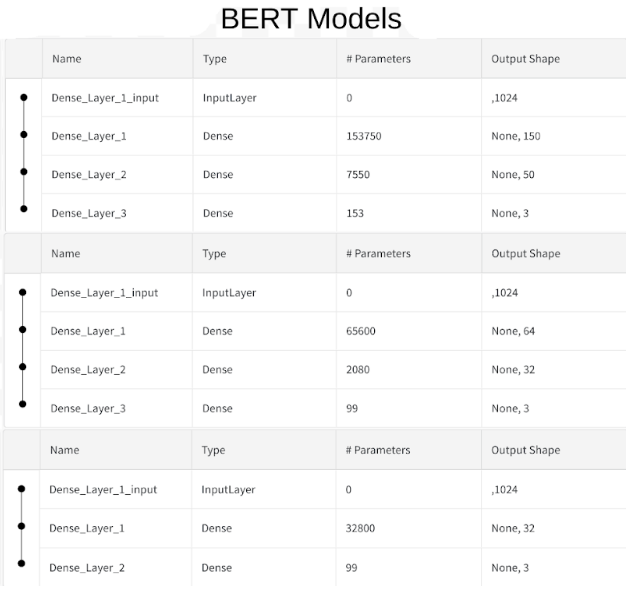
\includegraphics[width=\linewidth]{bert_model}
  \caption{BERT model configuration}
  \label{fig:bert_model}
  \end{subfigure}
\end{figure}


\section{Experiments}

    When we were ready to run the dataset consisting of one-hot encodings for the kingdom, and phylum corresponding with BERT and “keywords”/word embeddings representations through our classifying network, we decided to try multiple different feed-forward, dense, models to see how that would affect our results. Also, in order to organize each of these tests and store information on each of them, including the model weights for later test predictions, we used a python library and a corresponding website called “wandb”. The results for all of our tests can be found at \href{https://app.wandb.ai/art81/geneus}{https://app.wandb.ai/art81/geneus}. Essentially, we developed three different feed-forward, “classification” networks of varying complexities ranging from 2 hidden layers with 150, and 50 neurons, to 1 hidden layer with 32 neurons.

\section{Results}

\begin{table}[]
    \centering
    \begin{tabular}{|l|l|p{1cm}|p{1.5cm}|p{1.5cm}|}
    \hline
    \bfseries Model Name &
    \bfseries Accuracy &
    \bfseries Loss &
    \bfseries Validation Accuracy &
    \bfseries Validation Loss \\ \hline
Keyword \#1 &
0.9998 &
0.0016 &
0.9884 &
0.1099 \\ \hline
BERT \#1 &
0.9948 &
0.0209 &
0.9955 &
0.0323 \\ \hline
Keyword \#2 &
0.9999 &
0.0015 &
0.9888 &
0.1011 \\ \hline
BERT \#2 &
0.9952 &
0.0181 &
0.9973 &
0.0195 \\ \hline
Keyword \#3 &
0.9997 &
0.0009 &
0.9827 &
0.1255 \\ \hline
BERT \#3 &
0.9961 &
0.0145 &
0.9621 &
0.1541 \\ \hline
    \end{tabular}
    \caption{Corresponding model final results (decreasing model complexity down the table)}
    \label{fig:results}
\end{table}

The final model results can be seen in Table \ref{fig:results}.

\subsection{Evaluation on outside data}

\begin{table}
    \centering
    \begin{tabular}{|l|l|l|l|}
    \hline
    \: & \multicolumn{3}{c|}{\bfseries Predictions (Animal/Plant/Fungus)} \\ \hline
    \bfseries Model Name &
    \bfseries Animal &
    \bfseries Plant &
    \bfseries Fungus \\ \hline
Keyword \#1 &
1.0/0.0/0.0 &
0.0/1.0/0.0 &
0.0/0.0/1.0 \\ \hline
BERT \#1 &
1.0/0.0/0.0 &
0.0/1.0/0.0 &
0.0/0.0/1.0 \\ \hline
Keyword \#2 &
1.0/0.0/0.0 &
0.0/1.0/0.0 &
0.0/0.0/1.0 \\ \hline
BERT \#2 &
1.0/0.0/0.0 &
0.0/1.0/0.0 &
0.0/0.0/1.0 \\ \hline
Keyword \#3 &
0.95/0.05/0.0 &
0.0/1.0/0.0 &
0.0/0.0/1.0 \\ \hline
BERT \#3 &
1.0/0.0/0.0 &
0.0/0.96/0.04 &
0.0/0.03/0.97 \\ \hline

    \end{tabular}
    \caption{Results of evaluation of non-Wikipedia articles on various models. The model outputs are displayed as probabilities of animal, plant, and fungus, respectively.}
    \label{fig:evaluation}
\end{table}

We retrieved additional plant, animal, and fungus species descriptions from non-Wikipedia sources in order to test the representation that we had built. We found that all of the models continued to work quite well on these outside blurbs of text, scoring the correct results with high confidence as shown in Table \ref{fig:evaluation}.
\section{Conclusions}
We find that our two approaches worked well for the tasks we tested. Intuitively speaking, the distinction between animals, plants, and fungi should be dramatic enough to be relatively easy for a computer to distinguish. It would be interesting to test our pipeline on more granular taxonomic levels such as class, family, or even genus. One limitation in our current setup is that only a single Wikipedia article exists for each species, so as we increase the number of classes, we have fewer examples for each class. Another interesting variation would be to train our models on other text from other sources. Wikipedia has a distinctive encyclopedic writing style, and was used in the pre-training of both BERT and GLoVe. Our preliminary results on outside data suggest that the keyword approach is more robust to writing style than BERT embeddings. 

{
\bibliographystyle{ieee}
\bibliography{bibliography}
}

\end{document}
